\documentclass{article}
\usepackage{graphicx}
\usepackage{amsmath}
\usepackage[margin=1in]{geometry}
\usepackage{array}
\usepackage{listings}
\usepackage{xcolor}
\usepackage{tikz}
\usetikzlibrary{arrows}

\setlength{\parindent}{0pt}

\definecolor{codegreen}{rgb}{0,0.6,0}
\definecolor{codegray}{rgb}{0.5,0.5,0.5}
\definecolor{codepurple}{rgb}{0.58,0,0.82}
\definecolor{backcolour}{rgb}{0.95,0.95,0.92}

\lstdefinestyle{mystyle}{
	language=Java,
    backgroundcolor=\color{backcolour},
    commentstyle=\color{codegreen},
    keywordstyle=\color{blue},
    numberstyle=\tiny\color{codegray},
    stringstyle=\color{codepurple},
    basicstyle=\ttfamily,
    breakatwhitespace=false,
    breaklines=true,
    captionpos=b,
    keepspaces=true,
    numbers=left,
    numbersep=5pt,
    showspaces=false,
    showstringspaces=false,
    showtabs=false,
    tabsize=2
}

\lstset{style=mystyle}

\title{3S03 A2}
\author{Matthew Nesbitt, nesbim2, 400463297}
\date{February 2025}

\begin{document}
\maketitle
\section{Question 1}
\subsection{Part A}
There are two bugs I found in RomanNumerals. These bugs were identified using visual static analysis by reading through the code. I then
confirmed the bugs I had identified by running testcases that would exploit those faults to cause faulty output.
Firstly, an input of 9 results in "IVX", due to the final line in \lstinline{romanForDigit()} of
\lstinline{return "" + one + five + ten;}. This would be fixed by modifying this line to be \lstinline{return "" + one + ten;}. Secondly, There
is missing functionality for numbers beyond 9, where the values will begin wrapping back around to 0. This would be fixed by modifying the
line \lstinline{return romanForDigit(i, 'I', 'V', 'X');} to support the tens column by re-using the \lstinline{romanForDigit()} function
with different symbols: \lstinline{return romanForDigit(x, 'X', 'L', 'C') + romanForDigit(i, 'I', 'V', 'X');},
which would allow RomanNumerals to support input $0 \leq x \leq 99$.
\subsection{Part B}
Test cases available in q1.zip.\\
Test run success:\medskip \\
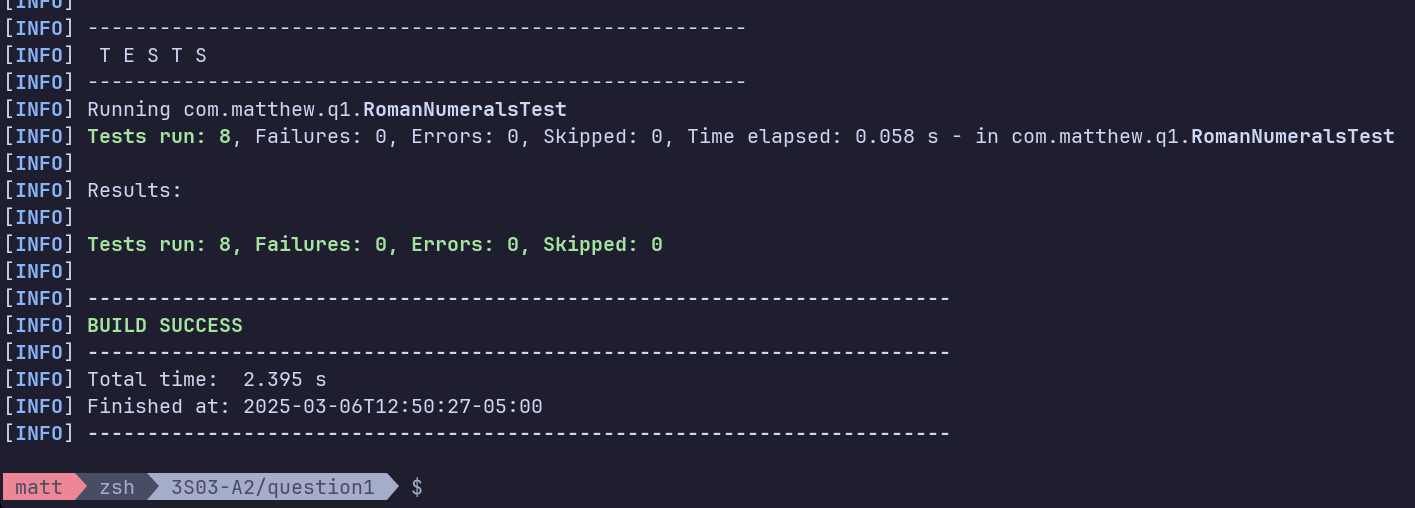
\includegraphics[scale=0.3]{tests.png}
\subsection{Part C}
A screenshot from SonarQube showing 100\% statement and 100\% condition coverage:\\
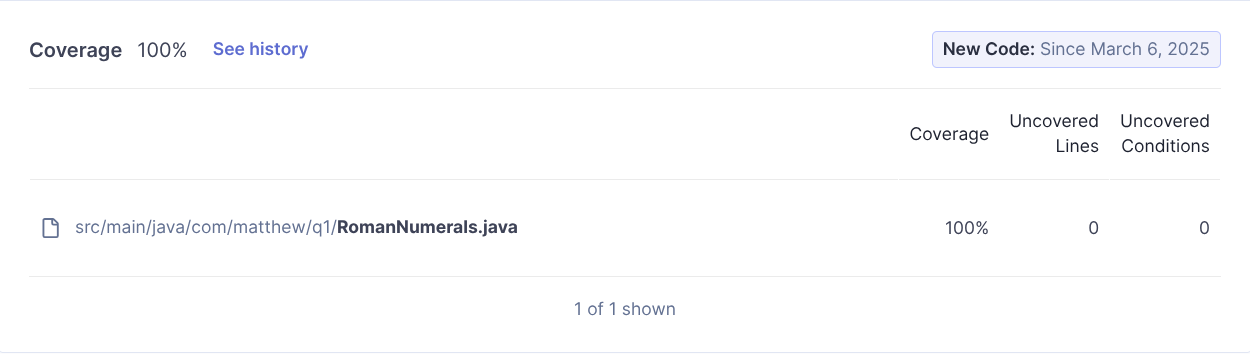
\includegraphics[scale=0.3]{sonarq.png}\\
A screenshot from the JaCoCo output file showing 100\% branch coverage:\\
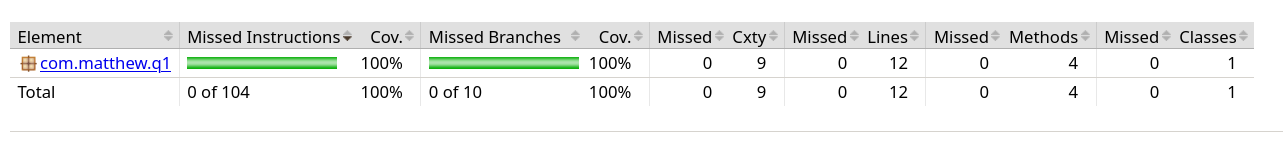
\includegraphics[scale=0.3]{jacoco.png}\\
My test suite also has 100\% MC/DC coverage as it meets all 4 required criteria:
\begin{itemize}
	\item 1: 100\% branch converage (shown in JaCoCo)
	\item 2: 100\% condition converage (shown in SonarQube)
	\item 3: As the only module is RomanNumerals, we cover the only entry point (\lstinline{RomanNumerals.roman()}) as well as the only exit point
		(\lstinline{RomanNumerals.roman()}).
	\item 4: Since every \lstinline{if} statement only has one condition, a change in that condition \textit{must} independently affect the output.
		Due to this, exercising every condition (condition converage) implies condition 4 for MC/DC.
\end{itemize}
\section{Question 2}
Test cases available in q2.zip.\medskip \\
In order to achieve a comprehensive test suite (excluding all exception paths), I used a combination of strong-normal partition testing, boundary testing, and edge cases.
Due to the nature of \lstinline{Min.min()}, accepting any comparable data type and any List implementation, the test suite can be broadly seperated into
two variables we can change: Comparable data type and List Implementation. Adhering to strong-normal partitioning principles for this, results in testing every data type
with every List implementation. For data types, I chose what I determined to be the most common use-cases for \lstinline{Min.min()}: Integers, Doubles, Characters,
and Strings. As for List implementations, I used all available List implementations listed on Oracle's website: ArrayList, LinkedList, and Vector. Each data type
were made their own set of tests, which were run on each List implementation.\medskip \\
For Integers, I partitioned the input space into positives and negatives. I then covered this space using a base case for positives and one for negatives, as well a boundary tests
for each partition. I tested the upper boundary for positives using \lstinline{Integer.MAX_VALUE}, the lower boundary for negatives using \lstinline{Integer.MIN_VALUE} and the boundary
about 0 by testing \lstinline{[-1, 0, 1]}. I then also tested all values being equal for positives, negatives and zero to uncover any odd behaviour on this edge case.\medskip \\
For Doubles, my testing methodology was identical to Integer, with some minor differences appearing in tests for the boundary about 0, where \lstinline{Double.MIN_VALUE} and
\lstinline{-Double.MIN_VALUE} are used for the positive and negative sides of the boundary respectively.\medskip \\
For Characters, partitioning into syntactically significant partitions is difficult, as all Characters are converted into positive ascii values for comparison. As such, I instead
made a \textit{semantic} distiction between upper-case letters, lower-case letters, digits and special characters to catch any unintentional case-flattening or automatic type-coercion within \lstinline{Min.min()}.
I intentionally do \textit{not} treat these as partitions, since they have no syntactic significance due to all being converted to positive integers as metioned above.
I also tested the edge case where all inputs are the same.\medskip \\
The same partitioning problem arises for Strings, and as such, I take a similar approach as I did with Characters. The primary difference here is that there is one
clear syntactically significant partition, being string length. To cover this partition I test a base case of regular length strings, and a lower boundary case of string length 0.
I do not test the upper boundary for this partition, as the theoretical upper boundary is \lstinline{Integer.MAX_VALUE}, but in practice is not consistent due to environmental and
computation limitations.\medskip \\
Finally, I test the lower boundary case for input List size of one (but ignore 0 as this is an invalid input) on all three List implementations. I do not test the upper boundary here
for the same reason as String length mentioned above.\medskip \\
\section{Question 3}
\subsection{Part A}
\textbf{Prompt:} Could you give me three reasons why I should use IEEE 829 to document my tests/testing?\medskip \\
\textbf{Response:}\\
IEEE 829 (also known as the Standard for Software and System Test Documentation) provides a structured approach to documenting software testing activities. Here are three reasons why you should consider using it:
\begin{itemize}
	\item \textbf{Consistency and Standardization}\\ IEEE 829 ensures that all test-related documents follow a uniform structure, making it easier to understand, review, and maintain.
		This is particularly useful in large teams or regulated industries where clear documentation is crucial.

	\item \textbf{Improved Traceability and Accountability}\\ The standard supports traceability by linking test cases to requirements, design specifications, and test results.
		This helps in tracking defects, ensuring complete coverage, and demonstrating compliance with industry regulations.

	\item \textbf{Better Communication and Collaboration}\\ Since IEEE 829 provides a clear framework for test plans, test cases, test reports, and other documents, it facilitates better
		communication among developers, testers, project managers, and stakeholders. This leads to more efficient testing and quicker resolution of issues.
\end{itemize}
Would you like a breakdown of specific IEEE 829 document types and how they fit into a project?
\subsection{Part B}
Many of its points are valid and have real value. As it states, having consistency and standardization to the structure of test-related documents can make a significant difference
to the organization and productivity of large teams working on complex projects. The same can be said for its other two points: They can definitely bring real-world benefits. The
glaring issue with this response, however, is the lack of specificity and instead just presenting generalized concepts that can be helpful. It doesn't bring any arguments as to why
one should use IEEE 829 \textit{specifically}, as opposed to any other testing standard or framework.
\subsection{Part C}
There are many reasons one may be inclined to use IEEE 829. To start, it provides a standardized set of \textit{integrity levels}, ranging from high integrity to low integrity. These integrity levels can help
you determine the relative importance of your software system in relation to all other software systems following this standard. Doing so helps you gauge your testing approach, and possibly compare with other
projects of a similar integrity level. Secondly, it provides \textit{Recommended minimum testing tasks for each integrity level}, which sets a minimum threshold of testing that your project should meet given
your integrity level. This is very helpful, as it provides a possible answer to the question of \textit{when to stop testing}, with reasonable authority. Finally, IEEE 829 provides a standard for creating a
Master Test Plan (MTP), which is used to describe and manage total test effort. This can be useful for coordinating/allocating effort between different teams/individuals to help achieve the desired testing outcome
with as much efficiency as possible.
\subsection{Part D}
\textbf{Prompt:} Could you give me three reasons why I shouldn't use IEEE 829 to document my tests/testing?\medskip \\
\textbf{Response:}\\
IEEE 829 (the Standard for Software Test Documentation) is a structured approach to test documentation, but it may not be ideal in some cases. Here are three reasons why you might not want to use it:
\begin{itemize}
	\item \textbf{Higher Maintenance Cost}\\ With extensive documentation requirements, IEEE 829 demands ongoing effort to update and maintain. As your project evolves, keeping test documents aligned with
		code changes can become a time-consuming task.

	\item \textbf{Limited Flexibility}\\ IEEE 829 enforces a rigid structure that might not suit all projects. If your testing approach is more exploratory, scriptless, or ad hoc,
		the structured documentation format may not align well with your workflow. This can lead to unnecessary work in documenting tests that don't fit neatly into IEEE 829’s templates.

	\item \textbf{Redundant or Unnecessary for Many Projects}\\ If your project already has well-defined test automation, clear user stories, and lightweight test documentation (e.g., in Jira, TestRail, or a similar tool),
		following IEEE 829 might duplicate efforts without adding much value. Many teams find that context-driven testing or risk-based testing is more practical than filling out extensive IEEE 829 documents.
\end{itemize}
Would you like suggestions for alternative test documentation approaches?
\subsection{Part E}
There are also many reasons teams may \textit{not} be inclined to use IEEE 829. Firstly, adhering to IEEE 829 may consume a large number of resources within your team, which may be better put to use actually
designing test suites or improving the product than filling out IEEE 829 documentation. Secondly, for systems like shrinkwrap which are non-critical, and need to quickly pivot to meet whatever the new trend is,
adhering to a structured test standard like IEEE 829 would likely not be necessary due to the low level of importance, and may prevent the team from making the quick pivots demanded by shrinkwrap software. Finally,
IEEE 829 is an aging standard in a rapidly changing industry. In many cases, IEEE 829 may not reccommend a reasonable course of action given new technologies created after IEEE 829. For this reason, many teams may
opt for another more modern standard (like IEEE 29119 mentioned in the question).
\end{document}
